% ======================================================================
% 第三部分：完成情况及性能参数
%   3.1 整体介绍
%   3.2 工程成果（3.2.1 机械成果、3.2.2 电路成果、3.2.3 软件成果）
%   3.3 特性成果（逐个展示功能、性能参数等量化指标，配仿真截图与图表）
% ======================================================================

\section{完成情况及性能参数}

\subsection{整体介绍}


本作品完成了赛题规定的五项核心功能、四项关键性能指标，以及官方 1022/1026/1030 答疑要求的 2 字节大端 VLID 顶层流式封装、$1\text{--}\MaxMessageBytes$~B IPv4 硬件自动分片和 \ReasmContexts{} 路并发按序重组。按官方答疑 R112，赛题无需硬件开发板上板，以 eLinx 3.0.7 综合布局布线、静态时序报告、VQM 门级网表后仿真及 ModelSim 波形作为考核依据。

图~\ref{fig:s3_elinx_ov} 中的 \code{Implementation Complete} 表示工程已完成布局布线。顶层 \code{AFDX_top} 的目标器件为 EQ6HL130-CSG484\_H；计入 0.30~ns 时钟不确定度后，96,142 个时序端点零违例，Setup 裕量为 +0.029~ns，Hold 裕量为 +0.604~ns。

\figWave[eLinx 3.0.7 工程综合与布局布线完成总览界面]{elinx_overview}{eLinx 3.0.7 布局布线结果：LUT 62,274（45.79\%）、FF 35,597（26.17\%）、I/O 172（50.74\%）、Memory 814（67.83\%）、CLB 10,230（75.22\%）}{fig:s3_elinx_ov}

表~\ref{tab:s3_compliance} 按赛题要求对照通信功能、性能与物理时序的实测结果。

\begingroup
\begin{longtable}{@{}>{\raggedright\arraybackslash}p{2.2cm}>{\raggedright\arraybackslash}p{3.3cm}>{\raggedright\arraybackslash}p{\dimexpr\linewidth-6.7cm-6\tabcolsep\relax}>{\centering\arraybackslash}p{1.2cm}@{}}
\caption{赛题要求与作品最终完成情况总览表}\label{tab:s3_compliance}\\
\longtablehead{4}{\thead{考核维度} & \thead{赛题与官方答疑规范要求} & \thead{作品实测结果与工程完成度} & \thead{结论}}
ARINC 664 P7 通信 & 128 TX / 4096 RX VL，BAG 调度，2B-VLID 流与 $1\text{--}8192$~B 分片重组 & 顶层 \code{AFDX_top} 支持 2B-VLID 流输入输出、128 TX / 4096 RX VL 线速处理、$1\text{--}\MaxMessageBytes$~B 自动 2--6 分片与 \ReasmContexts{} 路双 Bank 按序重组 & 符合 \\
高完整性通信 & 帧校验、每网独立 IC 序号检查、双网 RM 去重与异常统计 & 覆盖 FCS、帧长、IP/UDP 头、未知 VL、网络禁用、IC 乱序/重复、环形缓冲/队列/重组异常共 14 类检测计数与预写回退，双网先到先交付去重零差错 & 符合 \\
高层网络服务 & SNMP 网络管理、ARINC 615A 数据加载、RTC 时钟同步 & SNMPv1/v2c（Get/GetNext/Set/v2 Trap，36 项 MIB）、615A（TFTP 单文件上传与 MDD 下载，8~KiB RAM，双级 CRC-16）、SNTPv4（8~ns 分辨率，空载 0~ns 误差）闭环通过 & 符合 \\
有效载荷吞吐率 & $\ge 100$~Mbps（接收端去重后纯有效载荷） & 63~VL 满载规格单向达 \textbf{\ThruSixtyThree~Mbps}（双向 \textbf{\ThruSixtyThreeBi~Mbps}，为门限的 \textbf{7.41 倍}）；77/81~VL 压力下达 \textbf{\Thru/\ThruEightyOne~Mbps}，变长高负载 \ThruVarHigh~Mbps & 符合 \\
端到端传输时延 & $< 1\text{--}2$~ms（单帧 $\le 2000$~µs） & 顶层流口径：63~VL 周期最大 \textbf{\LatSixtyThreePMax~µs}，B2 两拍突发最大 \textbf{\LatSixtyThreeBTwo~µs}；核心流水口径：满载最大 \textbf{\Lat~µs}（评委入口 77~VL 全消息口径最大 48.600~µs） & 符合 \\
传输抖动控制 & $\le$几十微秒（同 VL 时延极差口径） & 定长发送间隔抖动 \textbf{\Jit~µs}；顶层 63~VL 周期 1471~B 抖动 \textbf{0.016~µs}（全包长 $\le\JitSixtyThreePer$~µs），B2 两拍突发 \textbf{\JitSixtyThreeBTwo~µs}（$<100$~µs）；核心定长同 VL 极差 \textbf{\JitSameVl~µs} & 符合 \\
物理时序与网表 & 125~MHz 静态时序收敛，门级网表与 RTL 一致 & 计入 \ClkUncert~ns 时钟不确定度后 \countsep{\RoutedEndpoints} 端点 0 违例，净 Setup \textbf{$+\RoutedSetup$~ns}（原始 $+\RoutedSetupRaw$~ns）、Hold \textbf{$+\RoutedHold$~ns}；4 类 VQM 门级网表后仿真通过 & 符合 \\
\end{longtable}
\endgroup

\subsection{工程成果}

\subsubsection{机械成果}

针对目标芯片 \textbf{EQ6HL130-CSG484\_H} 的 484 球 BGA 封装与片上阵列结构，工程完成了引脚锁定、物理簇锚定与 100\% 自动布线收敛（表~\ref{tab:s3_phys_layout}）：通过 \code{elinx/constraints.edc} 固定 \Pins{} 个用户 I/O 焊盘坐标，通过 \code{elinx/tiles_1030.edc} 锁定 \countsep{\LockedClusters} 个物理簇（\Clb{} 个 CLB 簇 $+$ \Mem{} 个 M4K 存储簇，0 缺失、0 坐标偏移），全芯片 64,939 条逻辑网络 100\% 布通，DRC 与布线冲突数为 0。

\begin{table}[H]\centering
\caption{芯片级物理版图锚定与布线实现成果（EQ6HL130-CSG484\_H）}\label{tab:s3_phys_layout}
\begin{tabularx}{\linewidth}{@{}>{\raggedright\arraybackslash}p{3.6cm}>{\raggedleft\arraybackslash}p{2.8cm}L@{}}
\toprule
\thead{物理版图与封装项目} & \thead{实现数值} & \thead{物理实现与约束审计结果} \\
\midrule
目标器件与封装形式 & EQ6HL130-CSG484\_H & 中科亿海微 eHiChip6 家族，484 球 BGA 封装（339 个可用用户 I/O） \\
顶层锁定用户引脚（P0 Pads） & \Pins{} / 339（\PinPct\%） & 172 条引脚位置约束 100\% 生效，涵盖双网 GMII、应用流、配置与事件口 \\
锁定 CLB 物理逻辑簇 & \Clb{} / 13,616（\ClbPct\%） & 按收发核心、32-Bank 映射表与 16 槽重组器分区紧凑锚定 \\
锁定 M4K 嵌入式存储簇 & \Mem{} / 1,200（\MemPct\%） & 承载 250 个同步 RAM 实例（4,174,544~bit），写口配 128 个写隔离 LUT \\
总锁定物理簇（\code{tiles_1030.edc}） & \countsep{\LockedClusters} 个簇 & 布局位置审计 0 缺失、0 漂移，CLI 与 GUI 布局布线产物逐字节一致 \\
全芯片物理布线网络数 & 64,939 条网络 & \code{PRES 1.30} 布局布线耗时 \ParElapsedSec~s，100\% 布通，0 未布通/0 重叠错误 \\
\bottomrule
\end{tabularx}
\end{table}

\subsubsection{电路成果}

\paragraph{（1）综合与布局布线后硬件资源占用及自研 MAC 优势对照}

在 eLinx 3.0.7 官方流程下，顶层 \code{AFDX_top}（\RtlFileCount{} 个 RTL 文件、\DesignUnitCount{} 个设计单元）布局布线后的硬件资源占用明细见表~\ref{tab:s3_synth_res}。

\begin{table}[H]\centering
\caption{整机综合与布局布线后资源占用表（EQ6HL130-CSG484\_H）}\label{tab:s3_synth_res}
\begin{tabularx}{\linewidth}{@{}>{\raggedright\arraybackslash}p{4.4cm}>{\raggedleft\arraybackslash}p{2.6cm}>{\raggedleft\arraybackslash}p{2.6cm}>{\raggedleft\arraybackslash}p{2.4cm}L@{}}
\toprule
\thead{硬件资源类别} & \thead{设计实际用量} & \thead{器件资源总量} & \thead{资源利用率} & \thead{备注说明} \\
\midrule
查找表（LUT） & \countsep{\Lut} & 136,160 & \LutPct\% & 含 128 个显式 \code{lut_mask="8888"} 写隔离 LUT \\
触发器（FF） & \countsep{\FF} & 136,160 & \FFPct\% & 含 \countsep{\MulticycleRegs} 个 \code{CE_DIV=2} 多周期引擎触发器 \\
可配置逻辑块（CLB） & \countsep{\Clb} & 13,616 & \ClbPct\% & 物理簇锁定于 \code{elinx/tiles_1030.edc} \\
片上嵌入式存储块（EBR / M4K） & \Mem & 1,200 & \MemPct\% & 映射 250 个同步 RAM（509.6~KiB），零寄存器阵列泄漏 \\
数字信号处理单元（DSP） / 锁相环（PLL） & 0 / 0 & 48 / 8 & 0.00\% & 纯数字逻辑与定点移位加减实现 \\
用户 I/O 引脚（Pins） & \Pins & 339 & \PinPct\% & 完整引出双网 GMII、2B-VLID 流、配置与统计端口 \\
\bottomrule
\end{tabularx}
\end{table}

同器件的单口资源对比见表~\ref{tab:s3_mac_cmp}。自研双网锁步 MAC 不仅实现了 0 拍空闲启动延迟与双网周期级严格同拍输出，而且完全不占用块 RAM，单口 LUT 与 FF 消耗仅为通用 IP 的 39.7\% 与 20.3\%。

\begin{table}[H]\centering
\caption{自研流式千兆 MAC 与官方 TripleSpeedEthernet IP 单口资源对比}\label{tab:s3_mac_cmp}
\begin{tabularx}{\linewidth}{@{}Lcccc@{}}
\toprule
\thead{实现方案} & \thead{查找表 (LUT)} & \thead{触发器 (FF)} & \thead{存储块 (M4K)} & \thead{可配置逻辑块 (CLB)} \\
\midrule
自研流式千兆 MAC（本设计） & \textbf{556}（39.7\%） & \textbf{198}（20.3\%） & \textbf{0}（0.0\%） & \textbf{69}（33.0\%） \\
eLinx 官方 TripleSpeedEthernet IP & 1,400（100\%） & 975（100\%） & 24（100\%） & 209（100\%） \\
\bottomrule
\end{tabularx}
\end{table}

\paragraph{（2）布局布线后全量静态时序分析（Post-Route STA）与门级网表后仿真成果}

在 125~MHz（8.000~ns 周期）并主动施加 \textbf{\ClkUncert~ns（\ClkUncertPs~ps）建立时间时钟不确定度（Clock Uncertainty）}的加严约束下，综合阶段与布局布线后的全量静态时序签核结果如表~\ref{tab:s3_sta} 所示。

\begin{table}[H]\centering
\caption{综合估算与布局布线后全量静态时序（Post-Route STA）签核对比表}\label{tab:s3_sta}
\begin{tabularx}{\linewidth}{@{}>{\raggedright\arraybackslash}p{4.3cm}>{\raggedleft\arraybackslash}p{2.9cm}>{\raggedleft\arraybackslash}p{3.0cm}L@{}}
\toprule
\thead{静态时序分析指标} & \thead{综合阶段估算} & \thead{布局布线后实测} & \thead{工程签核结论} \\
\midrule
主时钟周期 / 建立时间不确定度 & 8.000~ns / \ClkUncert~ns & 8.000~ns / \ClkUncert~ns & 125~MHz 全局单时钟，主动扣除 300~ps 不确定度 \\
8~ns 单周期最差净建立裕量 (WNS) & $+\Setup$~ns & \textbf{$+\RoutedSetup$~ns} & 269,131 条路径 0 违例（未扣不确定度原始裕量 \textbf{$+\RoutedSetupRaw$~ns}） \\
16~ns 多周期最差建立裕量 (\code{CE_DIV=2}) & --- & \textbf{$+\MulticycleSetup$~ns} & \MulticycleRules{} 条规则覆盖 \countsep{\MulticycleRegs} 个引擎触发器（50,050 条路径） \\
同沿最差保持时间裕量 (WHS) & $+\Hold$~ns & \textbf{$+\RoutedHold$~ns} & 319,181 条保持路径全部正裕量，TNS / THS 均为 0.000~ns \\
等效净最高工作频率 ($F_\text{max}$) & \Fmax~MHz & \textbf{\RoutedFmax~MHz} & 含不确定度净 $F_\text{max}$（原始物理 $F_\text{max}=\textbf{\RoutedFmaxRaw~MHz}$） \\
建立 / 保持时间违例端点数 & 0 / \countsep{\SynthEndpoints} & \textbf{0 / \countsep{\RoutedEndpoints}} & 全芯片所有同步时序终点 100\% 闭合 \\
\bottomrule
\end{tabularx}
\end{table}

表~\ref{tab:s3_crit} 列出决定最差裕量的路径。布局布线后，8~ns 最差路径的逻辑延迟为 1.423~ns，连线延迟为 6.173~ns。

\begin{table}[H]\centering
\caption{综合与布局布线后关键建立时间路径明细}\label{tab:s3_crit}
\setlength{\tabcolsep}{3.5pt}
\begin{tabularx}{\linewidth}{@{}>{\raggedright\arraybackslash}p{7.8cm}>{\centering\arraybackslash}p{1.0cm}>{\raggedleft\arraybackslash}p{1.4cm}>{\raggedleft\arraybackslash}p{1.4cm}>{\raggedleft\arraybackslash}X@{}}
\toprule
\thead{分析阶段与关键路径起点 $\rightarrow$ 终点} & \thead{逻辑级} & \thead{逻辑 (ns)} & \thead{连线 (ns)} & \thead{净裕量 (ns)} \\
\midrule
\textbf{[布线后 8~ns 最差]} \code{es|tx_core|engine|candidate/Q} $\rightarrow$ \code{es|cfg_regs|receive_bus[7].transmit_ack_q/D} & 3 & 1.423 & 6.173 & \textbf{$+\RoutedSetup$} \\
\textbf{[综合阶段 8~ns 最差]} \code{...reassembly...ram_block1a2~I|port_b_address_dff[0]/Q} $\rightarrow$ \code{...lanes[0].storage|read_result[0]~I|ff/D} & 2 & 3.108 & 0.000 & $+\Setup$ \\
\textbf{[布线后 16~ns 多周期最差]} \code{snmp_u / a615_u}（\code{CE_DIV=2}，50,050 条多周期内部路径） & --- & --- & --- & \textbf{$+\MulticycleSetup$} \\
\bottomrule
\end{tabularx}
\end{table}

导出的官方 VQM 门级网表在 ModelSim 下完成的 4 类后仿真验证结果见表~\ref{tab:s3_netlist}，门级网表输出与 RTL 参考记录 100\% 逐拍逐字节一致。

\begingroup
\setlength{\tabcolsep}{4pt}
\begin{longtable}{@{}>{\raggedright\arraybackslash}p{1.3cm}>{\raggedright\arraybackslash}p{3.9cm}>{\raggedright\arraybackslash}p{\dimexpr\linewidth-8.8cm-8\tabcolsep\relax}>{\raggedleft\arraybackslash}p{2.3cm}>{\centering\arraybackslash}p{1.3cm}@{}}
\caption{综合后 VQM 门级网表后仿真验证成果汇总}\label{tab:s3_netlist}\\
\longtablehead{5}{\thead{编号} & \thead{门级网表测试平台与耗时} & \thead{验证内容与 RTL 对照判据} & \thead{检查数/错误数} & \thead{结论}}
NET-01 & \code{tb_elinx}（耗时 \NetElinxTime~s） & 双端双网经顶层 2B-VLID 流互发 1/64/1471~B 消息并去重交付 & \ElinxChecks/0 & 通过 \\
NET-02 & \code{tb_net_services}（耗时 \NetCliTime~s） & 五项核心功能联合运行，7 份外部端口记录与 RTL 逐字节 SHA-256 完全一致 & \SvcChecks/0（自检）\newline 65/0（独立） & 通过 \\
NET-03 & \code{tb_frag1030_net}（耗时 \NetFragTime~s） & 分片与按序重组前 199,578 拍窗口（含复位初始化与 \code{VL 0x0102} 1472~B 两分片双网发送及重组），5 份文件 32 条记录与 RTL 一致 & 32/0 记录\newline 5/0 文件 & 通过 \\
NET-04 & \code{tb_t76_load}（TX \NetLoadTxTime~s / RX \NetLoadRxTime~s） & 顶层流包装 81~VL $+$ 1472~B 两分片混合窗口，收发两侧各 11 份记录与纯 RTL 逐字节相同，公开端口无 X/Z 态 & 161/0（TX）\newline 161/0（RX） & 通过 \\
\end{longtable}
\endgroup

\subsubsection{软件成果}

\textbf{eLinx 3.0.7 联调 ModelSim 行为仿真界面成果。}在 eLinx IDE 中一键执行 \code{Run Behavioral Simulation} 调用 ModelSim SE-64 2020.4 运行 \code{tb_elinx}，两个 \code{AFDX_top} 端系统经双网互发 1、64、1471 字节消息，图~\ref{fig:s3_welinx} 的日志窗口输出三行 \code{both_directions=PASS} 与 \code{[RESULT] tb_elinx PASS checks=9238 errors=0}。

\begin{figure}[H]\centering
\pgfmathsetlengthmacro{\zoomunit}{0.95*\linewidth/944}
\pgfmathsetlengthmacro{\overviewwidth}{0.54*\linewidth}
\pgfmathsetlengthmacro{\zoomimagewidth}{1309*\zoomunit}
\begin{tikzpicture}[x=\zoomunit,y=\zoomunit]
  \node[anchor=south,inner sep=0] at (472,222)
    {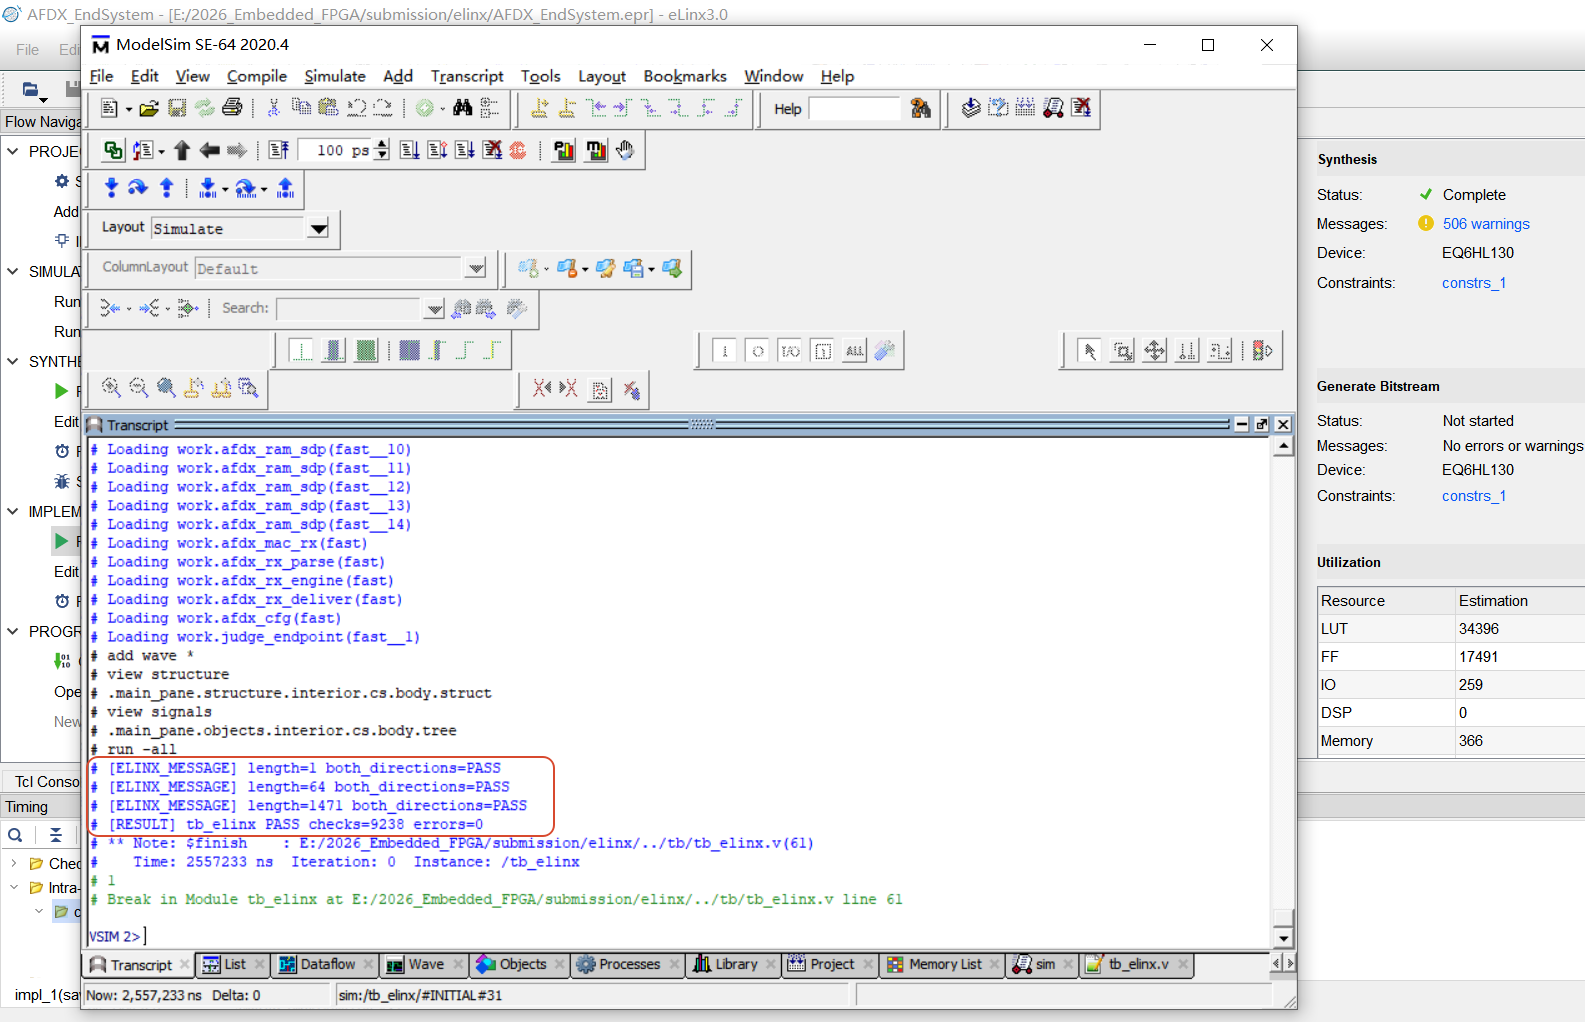
\includegraphics[width=\overviewwidth]{../../sim/wave/png/tb_elinx.png}};
  \draw[draw={rgb,255:red,197;green,80;blue,72},line width=0.6pt]
    (213.54,268.73) rectangle (600.51,355.63);
  \draw[draw={rgb,255:red,197;green,80;blue,72},line width=0.5pt]
    (213.54,268.73) -- (0,212);
  \draw[draw={rgb,255:red,197;green,80;blue,72},line width=0.5pt]
    (600.51,268.73) -- (944,212);
  \begin{scope}[overlay]
    \clip (0,0) rectangle (944,212);
    \node[anchor=south west,inner sep=0] at (-24,-114)
      {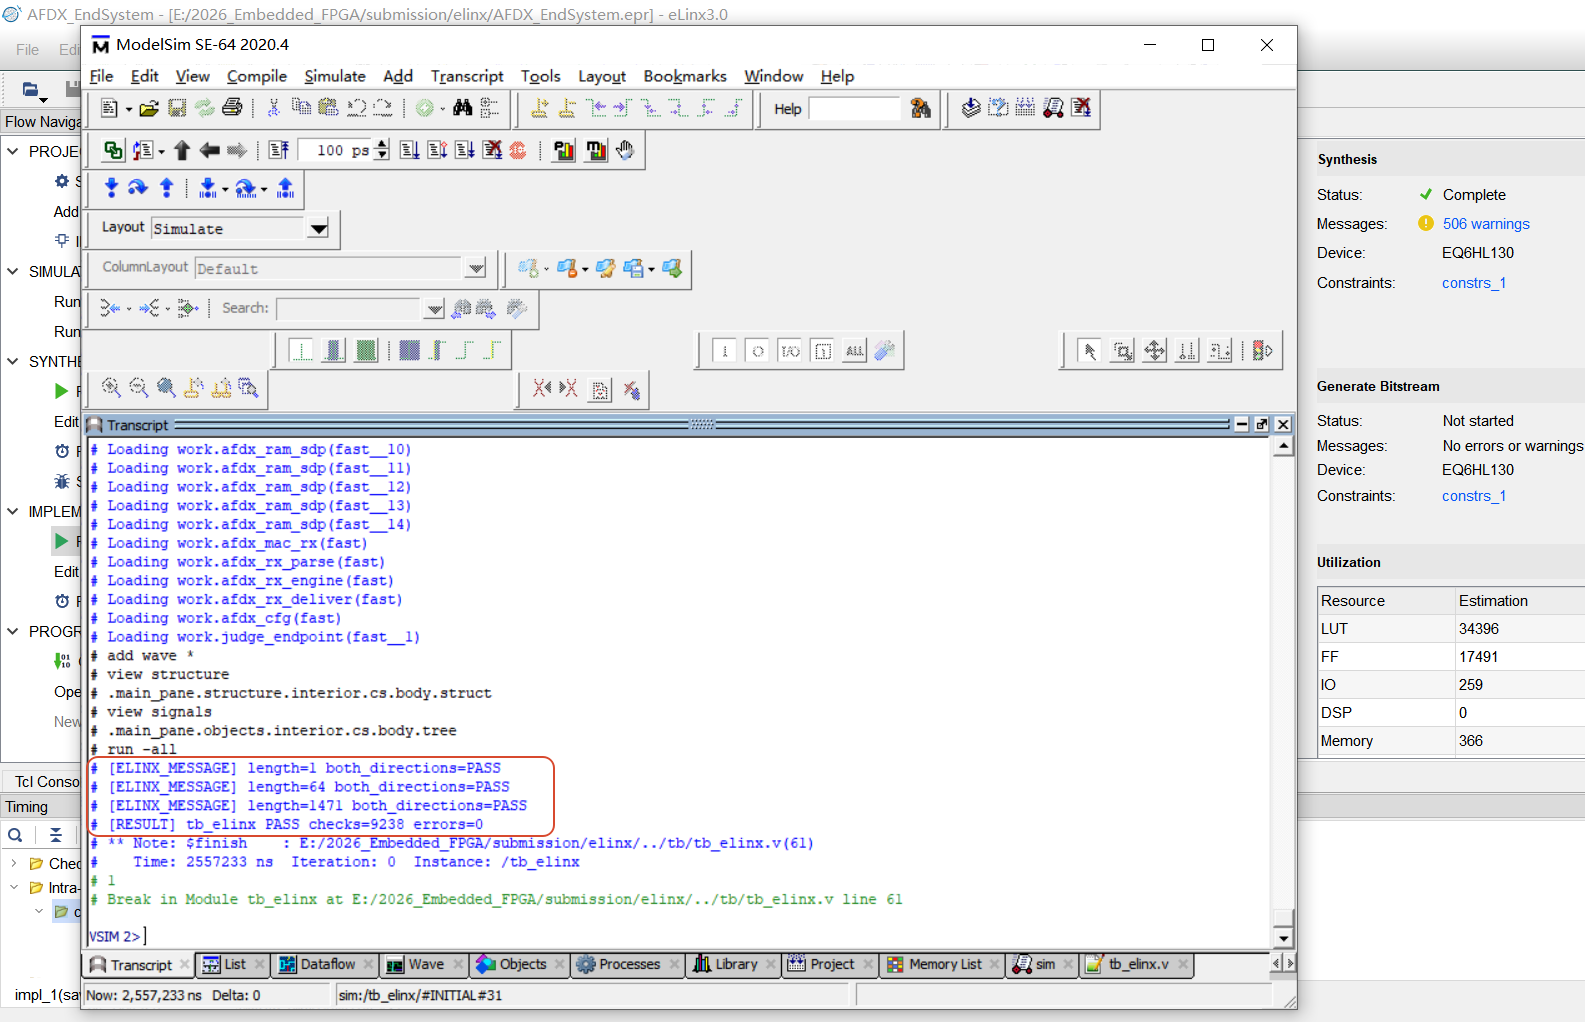
\includegraphics[width=\zoomimagewidth]{../../sim/wave/png/tb_elinx.png}};
  \end{scope}
  \draw[draw={rgb,255:red,197;green,80;blue,72},line width=0.6pt]
    (0,0) rectangle (944,212);
\end{tikzpicture}
\caption{eLinx 3.0.7 调用 ModelSim SE-64 2020.4 运行 \code{tb_elinx} 界面截图及底部 Transcript 日志放大图（\code{checks=9238 errors=0}）}\label{fig:s3_welinx}
\end{figure}

\textbf{评委一键入口 8 项全通过与五功能联合波形成果。}在分片交付版 RTL 上运行无 Python 依赖的评委入口 \code{do sim/run_judge.do}（归档于 \code{sim/reference/judge_result_frag1030.txt}），8 个系统级/性能评审用例全部输出 \code{JUDGE CASE PASS}（总运行时间约 2.3~h，累计完成 \textbf{1,949,513,089 次逐拍/逐字节在线断言检查、0 错误}）。评审用例与逐项检查数见表~\ref{tab:s3_judge}。

\begingroup
\begin{longtable}{@{}>{\raggedright\arraybackslash}p{2.1cm}>{\raggedright\arraybackslash}p{5.5cm}>{\raggedleft\arraybackslash}p{2.5cm}>{\raggedleft\arraybackslash}p{1.9cm}>{\centering\arraybackslash}p{\dimexpr\linewidth-12.0cm-8\tabcolsep\relax}@{}}
\caption{分片交付版评委入口（\code{sim/run_judge.do}）8 项核心评审用例实测汇总表}\label{tab:s3_judge}\\
\longtablehead{5}{\thead{评委用例名} & \thead{考核功能与核心实测指标（\code{judge_result_frag1030.txt}）} & \thead{逐拍/逐字节\newline 断言检查数} & \thead{实测耗时 (s)} & \thead{结论}}
\code{services} & 五项功能（用户收发、IC/RM、SNMP、RTC、615A 加载/卸载）联合自检 & 1,123 & 9.472 & PASS \\
\code{capacity} & 两端各配满 128 TX VL 与 4096 RX VL，抽样验证 0..4095 索引单次去重交付 & 49,924 & 13.669 & PASS \\
\code{snmp} & SNMPv1/v2c 的 Get、GetNext、Set 回写读回及 v2c Trap 启动通知 & 699 & 52.593 & PASS \\
\code{burst77} & 77 条最长帧（1471B）同拍突发排空：\code{queue_clear=983.720 µs} & 530,802 & 16.180 & PASS \\
\code{burst81} & 81 条最长帧（1471B）超规格突发排空：\code{queue_clear=1032.936 µs} & 554,734 & 17.325 & PASS \\
\code{rtc} & SNTP 对时误差：空载 \code{0 ns}，带载 \code{0 ns}，77~VL 满载最大 \code{8 ns} & 10,675,841 & 475.577 & PASS \\
\code{performance} & 77~VL 定长满载双向吞吐 \code{906.136 Mbps/方向}，全消息最大时延 \code{48.600 µs}（d257 为 \code{50.656 µs}），R119 同 VL 抖动 \code{0.008 µs} & 683,408,635 & 3,099.543 & PASS \\
\code{perf_var} & 多 VL 变长（\code{var_fixed/cycle/burst/high}）：\code{var_high} 双向各 \code{904.752 Mbps}、抖动 \code{0.008 µs}；\code{var_cycle} 最大抖动 \code{19.544 µs}（$<50$~µs） & 1,254,291,331 & 4,638.304 & PASS \\
\midrule
\textbf{8 项合计} & \textbf{\code{JUDGE ENTRY PASS cases=8}（Error=0, FAIL=0, RAMCOLL=0）} & \textbf{1,949,513,089} & \textbf{8,322.663} & \textbf{8/8 PASS} \\
\end{longtable}
\endgroup

图~\ref{fig:s3_services_wave} 可对照表中的 \code{services} 用例：从左至右读取 \code{phase}，可依次追踪用户数据、IC 坏序号拦截（\code{ic2=1}）、SNMP、RTC 对时（\code{difference=0 ns}）和 615A 加载成功（\code{status_value=2}）。双网去重计数为 \code{rm1/rm2=29}。

% ModelSim 截图以原始横向坐标对齐信号区与时间轴；只略去菜单及无信号空行。
% 两个位置参数为原图高度比例，分别表示信号区的下裁量、时间轴的上裁量。
\newsavebox{\waveSourceBox}
\newcommand{\waveWindow}[3]{%
  \sbox{\waveSourceBox}{\includegraphics{../../sim/wave/png/#1.png}}%
  \begingroup
  \edef\signalTrim{0pt \the\dimexpr#2\ht\waveSourceBox\relax\space 0pt \the\dimexpr.19\ht\waveSourceBox\relax}%
  \edef\axisTrim{0pt \the\dimexpr.045\ht\waveSourceBox\relax\space 0pt \the\dimexpr#3\ht\waveSourceBox\relax}%
  \edef\signalImage{\noexpand\includegraphics[width=.98\noexpand\linewidth,trim={\signalTrim},clip]{../../sim/wave/png/#1.png}}%
  \edef\axisImage{\noexpand\includegraphics[width=.98\noexpand\linewidth,trim={\axisTrim},clip]{../../sim/wave/png/#1.png}}%
  \vbox{\offinterlineskip
    \hbox{\signalImage}%
    \kern1pt
    \hbox{\axisImage}}%
  \endgroup}

\begin{figure}[H]\centering
\waveWindow{services}{.42}{.85}
\caption{五项功能联合测试（\code{tb_net_services}）的阶段与状态信号（ModelSim）}\label{fig:s3_services_wave}
\end{figure}

\textbf{全设计 \RtlFileCount{} 个 RTL 文件（\DesignUnitCount{} 个设计单元）代码覆盖率成果。}合并 \CovUcdbCount{} 份 UCDB 覆盖率库，全设计语句覆盖率达 \textbf{\CovStmt\%}（\CovStmtCov/\CovStmtTot）、分支覆盖率达 \textbf{\CovBranch\%}（\CovBranchCov/\CovBranchTot）、表达式覆盖率达 \textbf{\CovExpr\%}、FSM 状态覆盖率达 \textbf{\CovFsmState\%}（\CovFsmStateCov/\CovFsmStateTot，其中收发核心与全部高层服务主状态机均为 100.00\%）。各类覆盖率及未覆盖项见表~\ref{tab:s3_cov_sum}。

\begin{table}[H]\centering
\caption{全设计 \RtlFileCount{} 个 RTL 文件（\DesignUnitCount{} 个设计单元）ModelSim 代码覆盖率签核汇总（合并 \CovUcdbCount{} 份 UCDB）}\label{tab:s3_cov_sum}
\begin{tabularx}{\linewidth}{@{}lcccL@{}}
\toprule
\thead{覆盖率类别} & \thead{已覆盖项 / 总项数} & \thead{未覆盖项数} & \thead{实测覆盖率} & \thead{关键模块覆盖特征说明} \\
\midrule
语句覆盖率 (Statement) & \CovStmtCov{} / \CovStmtTot{} & 408 & \textbf{\CovStmt\%} & \code{AFDX_top}、\code{afdx_es}、\code{mac_rx}、\code{rx_core}、\code{tx_core} 等均为 100.0\% \\
分支覆盖率 (Branch) & \CovBranchCov{} / \CovBranchTot{} & 412 & \textbf{\CovBranch\%} & \code{afdx_app_tx} 达 99.81\%，\code{rx_engine} 达 98.96\%，\code{tx_engine} 达 98.38\% \\
表达式覆盖率 (Expression) & \CovExprCov{} / \CovExprTot{} & 745 & \textbf{\CovExpr\%} & \code{afdx_app_rx}、\code{mac_rx}、\code{mgmt_tx}、\code{tx_buf}、\code{tx_core} 均为 100.0\% \\
有限状态机状态 (FSM State) & \CovFsmStateCov{} / \CovFsmStateTot{} & 22 & \textbf{\CovFsmState\%} & 收发核心、MAC 及 RTC/SNMP/615A 服务引擎主状态机均为 \textbf{100.0\%} \\
条件覆盖率 (Condition) & \CovCondCov{} / \CovCondTot{} & 460 & \textbf{\CovCond\%} & 未命中项主要为双口 RAM 原语同址仿真保护与重组极端防卫分支 \\
信号翻转覆盖率 (Toggle) & \countsep{\CovToggleCov} / \countsep{\CovToggleTot} & 23,188 & \textbf{\CovToggle\%} & 未翻转位主要为 32 位异常计数器高 16 位及高序号重组缓存高位线 \\
\bottomrule
\end{tabularx}
\end{table}

\FloatBarrier
\subsection{特性成果}

以下逐项展示作品在五项核心功能、1026/1030 分片重组扩展以及吞吐率、时延、抖动、容量等量化指标上的测试成果与波形记录。

\paragraph{（1）ARINC 664 P7 双网锁步发送、BAG 调度与 $1\text{--}\MaxMessageBytes$~B IPv4 分片重组测试成果}

\textbf{双网同拍发送。}图~\ref{fig:s3_wtx} 先给出从应用口写入到双网 GMII 发送的信号顺序。

\figTest[应用消息与双网同拍发送矢量时序图]{t10_w_tx}{应用消息写入与 A、B 双网同拍发送 RTL 信号波形：(a) 应用口连续写入与调度；(b) 双网 GMII 同拍发出前导码与帧头}{fig:s3_wtx}

图~\ref{fig:s3_cap_tx} 的光标给出实测起点：A、B 两网在 \code{688.572 µs} 的同一时钟沿发出前导码 \code{0x55}。帧头仅第 11 字节源 MAC 接口号不同：A 网为 \code{0x20}，B 网为 \code{0x40}。

\begin{figure}[H]\centering
\waveWindow{tx_dual_1}{.54}{.85}\par\vspace{2pt}
{\footnotesize (a) 应用口写入与 A、B 双网同拍发送总览（光标 \code{688.572 µs} 处双网同步起始）\par}\vspace{4pt}
\waveWindow{tx_dual_2}{.54}{.85}\par\vspace{2pt}
{\footnotesize (b) 双网帧起点局部放大（前导码 \code{55}，源 MAC 网络接口号 A 网 \code{20}、B 网 \code{40}）\par}
\caption{应用消息与 A、B 双网同拍发送的 ModelSim 原始波形截图}\label{fig:s3_cap_tx}
\end{figure}

\textbf{BAG 最小间隔。}图~\ref{fig:s3_cap_bag} 中，同一 VL 相邻两帧的发送起点为 \code{17.132 µs} 与 \code{817.132 µs}。两光标相差 \code{800.000 µs}（100,000 拍），等于配置的 BAG；稳态发送间隔抖动为 \textbf{0.000~µs}。

\begin{figure}[H]\centering
\waveWindow{tx_bag}{.59}{.83}
\caption{同一 VL 两帧发送起点的 BAG 间隔测量（ModelSim）}\label{fig:s3_cap_bag}
\end{figure}

\textbf{8192 字节超长消息 6 分片发送与按序重组实测波形。}针对官方 1030 答疑 R138/R139，图~\ref{fig:s3_cap_frag} 展示了 \code{VL 0x0103} 单条 $8192$~B 最长应用消息的 ModelSim 实测波形（\code{sim/wave/frag.do}）：发送端自动拆分为 6 个 IPv4 分片帧（IP 片偏移依次为 0、1472、2944、4416、5888、7360 字节，前 5 片 \code{MF=1}、末片 \code{MF=0}，图~\ref{fig:s3_cap_frag}c 光标处首片 IP 标志与偏移字段为 \code{20 00}），相邻分片严格间隔 1~ms BAG 从 A、B 双网同拍发出（图~\ref{fig:s3_cap_frag}a）；第 6 片（末片）于 \code{5657.028 µs} 到达后，接收端在 \code{5671.524 µs} 启动连续无反压输出，一次完整交付 \code{8194} 字节（2B 大端 VLID $+$ 8192B 载荷，图~\ref{fig:s3_cap_frag}b），从应用首字节输入（\code{524.768 µs}）至末字节交付结束（\code{5737.076 µs}）总耗时 \code{5212.308 µs}，与输入逐字节 100\% 一致。

\begin{figure}[H]\centering
\waveWindow{frag_1}{.47}{.77}\par\vspace{2pt}
{\footnotesize (a) \code{VL 0x0103} 单条 8192~B 消息拆分为 6 个 IPv4 分片帧（间隔 1~ms BAG）及完整重组交付总览（全程 \code{5212.308 µs}）\par}\vspace{4pt}
\waveWindow{frag_2}{.47}{.77}\par\vspace{2pt}
{\footnotesize (b) 末片到达（\code{5657.028 µs}）后接收端开始连续交付（\code{5671.524 µs}），\code{rx_bytes} 计满 \code{8194} 字节（2B VLID + 8192B 载荷）\par}\vspace{4pt}
\waveWindow{frag_3}{.47}{.79}\par\vspace{2pt}
{\footnotesize (c) 首分片 IP 头字节局部放大（光标 \code{657.252 µs} 处 IPv4 标志与片偏移字段为 \code{20 00}，即 \code{MF=1}、偏移 0）\par}
\caption{8192 字节超长消息 IPv4 6 分片发送与接收端按序重组的 ModelSim 原始波形截图}\label{fig:s3_cap_frag}
\end{figure}

\FloatBarrier
\paragraph{（2）高完整性通信（IC 序号检查、双网 RM 去重与 14 类异常统计）测试成果}

\textbf{IC 序号状态转移与双网独立 PSN 验证。}在用例 RX-03 中，注入序号 7、8（步进 1）、10（步进 2，容忍单帧丢失）均被接纳；注入序号 13（步进 3）被 IC 拒绝但同步更新本网 PSN 为 13，使随后到达的序号 14 立即恢复接纳，而重复注入的序号 14（步进 0）被准确拒绝；A、B 两网 PSN 状态完全独立。其接纳、拒绝及两网独立更新过程见图~\ref{fig:s3_ic_seq}。

\figTest[IC 序号判决与双网独立状态更新验证图]{t03_ic_sequence}{IC 序号完整性判决与双网状态更新实测：(a) 同网连续、丢一帧容忍、跳号拒绝后立即同步及重复帧拦截；(b) A、B 两网独立维护 PSN 状态}{fig:s3_ic_seq}

\textbf{双网去重。}图~\ref{fig:s3_cap_rm} 中，先到的 A 网副本于 \code{3016.844 µs} 交付应用（\code{app_rx_net=0}）。B 网副本晚到 \code{15.784 µs}，在 \code{3032.628 µs} 被共享 RM 模块丢弃，并触发 \code{ev_rm_drop}。

\begin{figure}[H]\centering
\waveWindow{rx_redundancy_1}{.52}{.83}\par\vspace{2pt}
{\footnotesize (a) 先到的 A 网有效副本触发交付事件并输出应用载荷（光标 \code{3016.844 µs}）\par}\vspace{4pt}
\waveWindow{rx_redundancy_2}{.52}{.83}\par\vspace{2pt}
{\footnotesize (b) 晚到的 B 网同序号副本被冗余管理（RM）丢弃并触发 \code{ev_rm_drop}（光标 \code{3032.628 µs}）\par}
\caption{双网冗余副本先到交付与晚到去重的 ModelSim 原始波形截图}\label{fig:s3_cap_rm}
\end{figure}

\textbf{FCS 错误与单网容错。}图~\ref{fig:s3_cap_fcs} 中，A 网 FCS 错帧使 \code{count_a_fcs} 由 0 增至 1，B 网完好副本仍正常交付。主机从配置口读取地址 \code{0x49}，两拍后返回计数值 1。

\begin{figure}[H]\centering
\waveWindow{rx_fcs_error_1}{.45}{.85}\par\vspace{2pt}
{\footnotesize (a) A 网副本检测出 FCS 错误被拒收（\code{count_a_fcs} 增至 1），B 网完好副本正常交付\par}\vspace{4pt}
\waveWindow{rx_fcs_error_3}{.59}{.80}\par\vspace{2pt}
{\footnotesize (b) 主机配置口在 \code{973.404 µs} 读取地址 \code{0x49}，两拍后（\code{973.420 µs}）返回 \code{cfg_rdata=1}\par}
\caption{FCS 错误帧检测、单网容错交付与配置总线读回的 ModelSim 原始波形截图}\label{fig:s3_cap_fcs}
\end{figure}

表~\ref{tab:s3_fault14} 将这一方法扩展到 14 类异常：对照注入位置、样本数与寄存器读回值，可分别核查发送拒绝、接收回退和重组槽回收。

\begingroup
\setlength{\tabcolsep}{3.5pt}
\begin{longtable}{@{}>{\raggedright\arraybackslash}p{2.3cm}>{\raggedright\arraybackslash}p{1.6cm}>{\raggedright\arraybackslash}p{5.5cm}>{\raggedright\arraybackslash}p{\dimexpr\linewidth-9.4cm-6\tabcolsep\relax}@{}}
\caption{收发全通路 14 类异常故障注入与统计寄存器读回验证汇总}\label{tab:s3_fault14}\\
\longtablehead{4}{\thead{异常类别} & \thead{测试用例} & \thead{故障注入方式与样本规模} & \thead{硬件处置行为与配置口寄存器读回结果}}
发送 VL 禁用 & SYS-04 & 向未启用 VL 125 提交 1 条消息 & 拒绝入队、回滚页，\code{0x41 (drop_dis) = 1} \\
发送队列已满 & SYS-04 & 向 \code{qmax=0} 的 VL 127 提交 1 条消息 & 拒绝入队、回滚页，\code{0x42 (drop_full) = 1} \\
发送消息超长 & SYS-04 & 向 \code{max_payload=1} 的 VL 126 提交 18B 消息 & 回滚全部已占页并排空残余字节，\code{0x43 (drop_long) = 1} \\
发送无空闲页 & SYS-04 & 85 条长包占满 255 页后提交 1471/512/1B 消息 & 跨页无页立即退回首占页供 512B 复用，\code{0x44 (drop_nopage) = 2} \\
接收 FCS 错误 & SYS-02 & 改写帧字节，每端每网注入 2 帧（共 8 帧） & \code{mac_rx} 整帧丢弃，每端 \code{0x49/0x51 = 2/2} \\
接收帧长错误 & SYS-02 & 插入截短/超长帧，每端每网 1 帧（共 4 帧） & \code{mac_rx} 整帧丢弃，每端 \code{0x4a/0x52 = 1/1} \\
接收 IP 头错误 & SYS-02 & 插入版本/校验和错误 IP 帧，每端每网 1 帧 & \code{rx_parse} 回退 \code{trial} 指针，每端 \code{0x4b/0x53 = 1/1} \\
接收 UDP 头错误 & SYS-02 & 插入非零错误 UDP 校验和帧，每端每网 1 帧 & \code{rx_parse} 回退 \code{trial} 指针，每端 \code{0x4b/0x53} 累加至 \code{2/2} \\
接收未知 VLID & SYS-02 & 注入未映射 VLID 帧，每端每网 1 帧 & \code{rx_engine} 回退 \code{trial} 指针，每端 \code{0x4c/0x54 = 1/1} \\
接收网络不允许 & SYS-02 & 注入单网禁用副本，每端 A/B 各 1 帧 & \code{rx_engine} 回退 \code{trial} 指针，每端 \code{0x4d/0x55 = 1/1} \\
IC 同网序号重复 & SYS-02 & 四条单向链路各重放 1 帧同 SN 报文 & \code{rx_engine} IC 拦截回退，每端 \code{0x4e/0x56 = 1/1} \\
IC 同网序号乱序 & SYS-02 & 四条单向链路各延后重放旧 SN 报文 & \code{rx_engine} IC 拦截并更新 PSN，每端 \code{0x4e/0x56} 累加至 \code{2/2} \\
接收环形缓冲溢出 & SYS-07 & 环形缓冲缩至 512B，注入 513/1000/1471B 帧 & 空间不足不写入、短帧正常穿插交付，每端 \code{0x4f/0x57 = 3/3} \\
交付队列/重组拒绝 & RX-06/FRAG & 队列缩至 2 项注入 8 帧；注入乱序/缺首片/超 8192B 分片 & 队列满丢弃 1 次、去重 2 次、交付 5 条；异常分片立即回收重组槽 \\
\end{longtable}
\endgroup

\paragraph{（3）SNMP 网络管理、ARINC 615A 软件数据加载与 RTC 时钟同步测试成果}

\textbf{SNMPv1/v2c 查询、设置与 Trap 通知。}通过 \code{pyasn1} 独立验证 36 个 MIB 对象的 v1/v2c Get 精确查询与 GetNext 全表遍历、\code{USER_ID} 读写 Set 与非法写入拦截（只读对象返回 \code{noSuchName=2} 或 \code{notWritable=17}，类型不符返回 \code{badValue=3} 或 \code{wrongType=7}），以及 \code{coldStart} 与 \code{authenticationFailure} 两类 SNMPv2-Trap 报文上报。图~\ref{fig:s3_cap_snmp} 展示了 Get 请求在 \code{525.964 µs} 到达、代理在 \code{538.628 µs}（相距 \code{12.664 µs}）从双网同步发出 GetResponse 的 ModelSim 原始波形。

\begin{figure}[H]\centering
\waveWindow{snmp_get_1}{.54}{.83}\par\vspace{2pt}
{\footnotesize (a) SNMP Get 请求经 A、B 双网到达代理（光标 \code{525.964 µs}）\par}\vspace{4pt}
\waveWindow{snmp_get_2}{.54}{.83}\par\vspace{2pt}
{\footnotesize (b) 代理完成 BER 解码与 MIB 读取后从 A、B 双网同步发出 GetResponse（光标 \code{538.628 µs}，响应耗时 \code{12.664 µs}）\par}
\caption{SNMP Get 请求到达与双网同步响应的 ModelSim 原始波形截图}\label{fig:s3_cap_snmp}
\end{figure}

\textbf{ARINC 615A 软件数据加载与介质定义卸载。}完整通过 1500~B（短末块）与 1536~B（512~B 整倍数补零长末块）上传/卸载、单次丢包超时重传恢复、DATA2 比特翻转 CRC-16 拦截（上报 \code{STATUS=0x0303}）、重传耗尽终止（\code{STATUS=0x0503}）、A4/A3 版本兼容与 A5 非法版本拒绝、RFC 2347 扩展选项忽略等 6 大场景，主机读回的 8~KiB 加载 RAM 与 MDD 回传的 \code{MEMORY.BIN} 均与源文件 100\% 逐字节吻合。图~\ref{fig:s3_w615a} 给出 TFTP 数据块与双网确认时序。

\figTest[ARINC 615A TFTP 数据块传输与确认时序图]{t15_w_615a}{ARINC 615A 目标端 TFTP 数据块接收、双网 ACK 确认与短末块结束传输时序}{fig:s3_w615a}

\textbf{RTC 纳秒级时钟同步。}空载 20 次同步最大误差为 \textbf{\RtcIdle~ns}（评委入口 \code{rtc} 用例在空载与普通带载下均为 \textbf{0~ns}，77~VL 满载下最大误差仅 \textbf{8~ns}；长时带载极限包碰撞下最大误差为 \RtcLoad~ns $=10.788$~µs，小于单帧 12.304~µs 传输时长），并完整通过丢包重发与过期 Originate 防误校测试。请求、应答及校时的先后关系见图~\ref{fig:s3_wrtc}。

\figTest[SNTPv4 时钟同步请求与响应时序图]{t16_w_rtc}{RTC 时钟同步 SNTPv4 客户端请求、服务端回显 Originate 时间戳与本地时钟校准时序}{fig:s3_wrtc}

\FloatBarrier
\paragraph{（4）吞吐率、端到端时延、R97/R119 传输抖动与突发容量量化指标成果}

\textbf{顶层 \code{AFDX_top} 63-VL 声明满载规格与混合分片实测。}在 100~ms 双向双网窗口内，63 条 VL 满载（\code{P1471}）单向去重有效吞吐率达 \textbf{\ThruSixtyThree~Mbps}（双向合计 \textbf{\ThruSixtyThreeBi~Mbps}），最大端到端时延 \textbf{\LatSixtyThreePMax~µs}，同 VL 极差抖动仅 \textbf{0.016~µs}（跨 $1\text{--}1471$~B 五档周期工况最大抖动 $\le\JitSixtyThreePer$~µs）；背靠背两拍轮换突发（\code{B2}）最大时延 \textbf{\LatSixtyThreeBTwo~µs}（$<2000$~µs）、BAG 等待抖动 \textbf{\JitSixtyThreeBTwo~µs}（$<100$~µs）；63~VL 混合单帧与 1472/3000/8192~B 分片长消息（\code{mixed_profile}）双向无损交付 \textbf{12,206 条消息}，0 丢包、0 错包。各工况见表~\ref{tab:s3_perf63}。

\begin{table}[H]\centering
\caption{顶层 \code{AFDX_top} 63-VL 声明满载规格 7 组定长工况与混合分片实测结果（100~ms 双向双网）}\label{tab:s3_perf63}
\setlength{\tabcolsep}{3.5pt}
\begin{tabularx}{\linewidth}{@{}>{\raggedright\arraybackslash}p{2.5cm}>{\raggedleft\arraybackslash}p{2.2cm}>{\raggedleft\arraybackslash}p{2.2cm}>{\raggedleft\arraybackslash}p{2.4cm}>{\centering\arraybackslash}p{1.8cm}>{\raggedleft\arraybackslash}p{1.6cm}>{\centering\arraybackslash}X@{}}
\toprule
\thead{测试场景 / 载荷} & \thead{双向总吞吐\newline (Mbps)} & \thead{最大端到端\newline 时延 (µs)} & \thead{同 VL 最大\newline 抖动 (µs)} & \thead{页池峰值\newline 占用} & \thead{仿真耗时\newline (s)} & \thead{结论} \\
\midrule
\code{P1}（1~B 周期） & 1.008 & 38.440 & 2.016（\code{0x0104}） & 57 / 256 & 740.3 & PASS \\
\code{P17}（17~B 周期） & 17.136 & 34.600 & \textbf{\JitSixtyThreePer}（\code{0x0104}） & 51 / 256 & 751.5 & PASS \\
\code{P256}（256~B 周期） & 258.048 & 41.360 & 0.016（\code{0x010E}） & 16 / 256 & 905.0 & PASS \\
\code{P1024}（1024~B 周期） & 1,032.192 & 65.984 & 0.008（\code{0x0100}） & 14 / 256 & 1,394.5 & PASS \\
\code{P1471}（1471~B 满载） & \textbf{\ThruSixtyThreeBi} & \textbf{\LatSixtyThreePMax} & \textbf{0.016}（\code{0x0100}） & 18 / 256 & 1,418.6 & PASS \\
\code{B1}（1471~B 固定两拍突发） & 1,477.415 & \LatBOne & ---\textsuperscript{*} & 144 / 256 & 1,649.4 & PASS \\
\code{B2}（1471~B 轮换两拍突发） & 1,477.119 & \textbf{\LatSixtyThreeBTwo} & \textbf{\JitSixtyThreeBTwo}（\code{0x0114}） & 156 / 256 & 1,411.6 & PASS \\
\code{mixed_profile}（混合分片） & 60 短 $+$ 3 分片 & 8192B: 5,212.3 & 单帧 $\le 3.360$ & $\le 205 / 256$ & 12,206 条 & PASS \\
\bottomrule
\end{tabularx}
\par\vspace{2pt}\raggedright\footnotesize
注：\textsuperscript{*}\code{B1} 按固定 VL 次序连续注入两帧，3,150 对消息全部通过 BAG 最小间隔与逐字节核对；跨帧抢占下的 BAG 等待抖动由每三相邻 VL 轮换注入次序的 \code{B2} 测量。
\end{table}

\textbf{超规格工况的有效吞吐。}77~VL 与 81~VL 的单向有效吞吐分别为 \textbf{\Thru~Mbps} 与 \textbf{\ThruEightyOne~Mbps}。80~VL 变长高负载（\code{var_high}）下，单向为 \textbf{\ThruVarHigh~Mbps}，双向合计 1809.504~Mbps。图~\ref{fig:s3_thru} 将不同规模与 100~Mbps 赛题门限并列。

\figTest{t20_thru}{不同活跃 VL 规模下的单向有效载荷吞吐率与 100~Mbps 赛题门限对比}{fig:s3_thru}

\textbf{时延与抖动。}内核定长满载（\code{gbe77_d0}）下，单帧提交至末字节交付最大时延为 \textbf{\Lat~µs}，同 VL 抖动仅 \textbf{\JitSameVl~µs}（1 拍）。图~\ref{fig:s3_lat} 按阶段拆解 1471~B 帧的时延；评委入口按全消息统计，\code{max_e2e_us} 为 \textbf{48.600~µs}。

\figTest{t21_lat}{端到端时延与帧长关系及 1471~B 满载帧 3053 拍（24.424~µs）流水拆解}{fig:s3_lat}

\textbf{突发排空。}77 条与 81 条最长帧同拍突发在顶层流接口下的排空时间分别为 \textbf{\BurstSevSeven~µs} 和 \textbf{\BurstEightOne~µs}（评委入口实测 983.720~µs 与 1032.936~µs），均小于 2~ms 门限。内核各工况的分段时延、全消息时延与抖动见表~\ref{tab:s3_perf_core}。

\begingroup
\tablestyle
\setlength{\tabcolsep}{3.2pt}
\begin{longtable}{@{}>{\raggedright\arraybackslash}p{2.2cm}>{\raggedleft\arraybackslash}p{1.8cm}>{\raggedleft\arraybackslash}p{1.6cm}>{\raggedleft\arraybackslash}p{2.3cm}>{\raggedleft\arraybackslash}p{2.3cm}>{\raggedleft\arraybackslash}p{1.8cm}>{\raggedleft\arraybackslash}p{\dimexpr\linewidth-12cm-12\tabcolsep\relax}@{}}
\caption{内核多工况分段时延、全消息时延（分片版评委基准）与抖动实测汇总表}\label{tab:s3_perf_core}\\
\longtablehead{7}{\thead{测试工况} & \thead{单向吞吐\newline (Mbps)} & \thead{$L_\text{tx}$ 基线\newline (µs)} & \thead{$L_\text{rx}$ 首/末\newline (µs)} & \thead{$L_\text{app}$ 基线 / 全消息\newline 最大时延 (µs)} & \thead{R97 / R119\newline 抖动 (µs)} & \thead{发送间隔\newline 偏差 (µs)}}
\code{gbe77_d0} & \textbf{906.136} & 0.312 & 12.360 / 24.120 & 24.432 / \textbf{48.600} & \textbf{0.008} & 0.000 \\
\code{gbe77_d257} & \textbf{906.136} & 0.312 & 12.360 / 24.120 & 26.488 / \textbf{50.656} & \textbf{0.008} & 0.000 \\
\code{gbe81_d0} & \textbf{953.208} & 0.312 & 12.360 / 24.120 & 24.432 / --- & \textbf{0.008} & 0.000 \\
\code{fe10_d0} & 117.680 & 1.880 & 121.648 / 133.408 & 135.288 / --- & 0.000 & 0.000 \\
\midrule
\code{var_fixed_d0} & 57.794 & 0.360 & 12.360 / 24.120 & 24.432 / 48.600 & 0.008 & 0.000 / 0.008 \\
\code{var_cycle_d0} & 70.403 & 12.216 & 12.352 / 24.112 & 24.424 / 48.592 & 9.992 / 19.544 & 6.192 / 12.352 \\
\code{var_high_d0} & \textbf{904.752} & 12.016 & 12.360 / 24.120 & 24.432 / \textbf{48.600} & \textbf{0.008} & 0.000 / 0.016 \\
\code{var_burst_d0} & 57.794 & 21.128 & 12.352 / 24.112 & 32.888 / 63.256 & 0.000 / 0.008 & 0.000 \\
\end{longtable}
\endgroup
